

\tikzset{every picture/.style={line width=0.75pt}} %set default line width to 0.75pt        

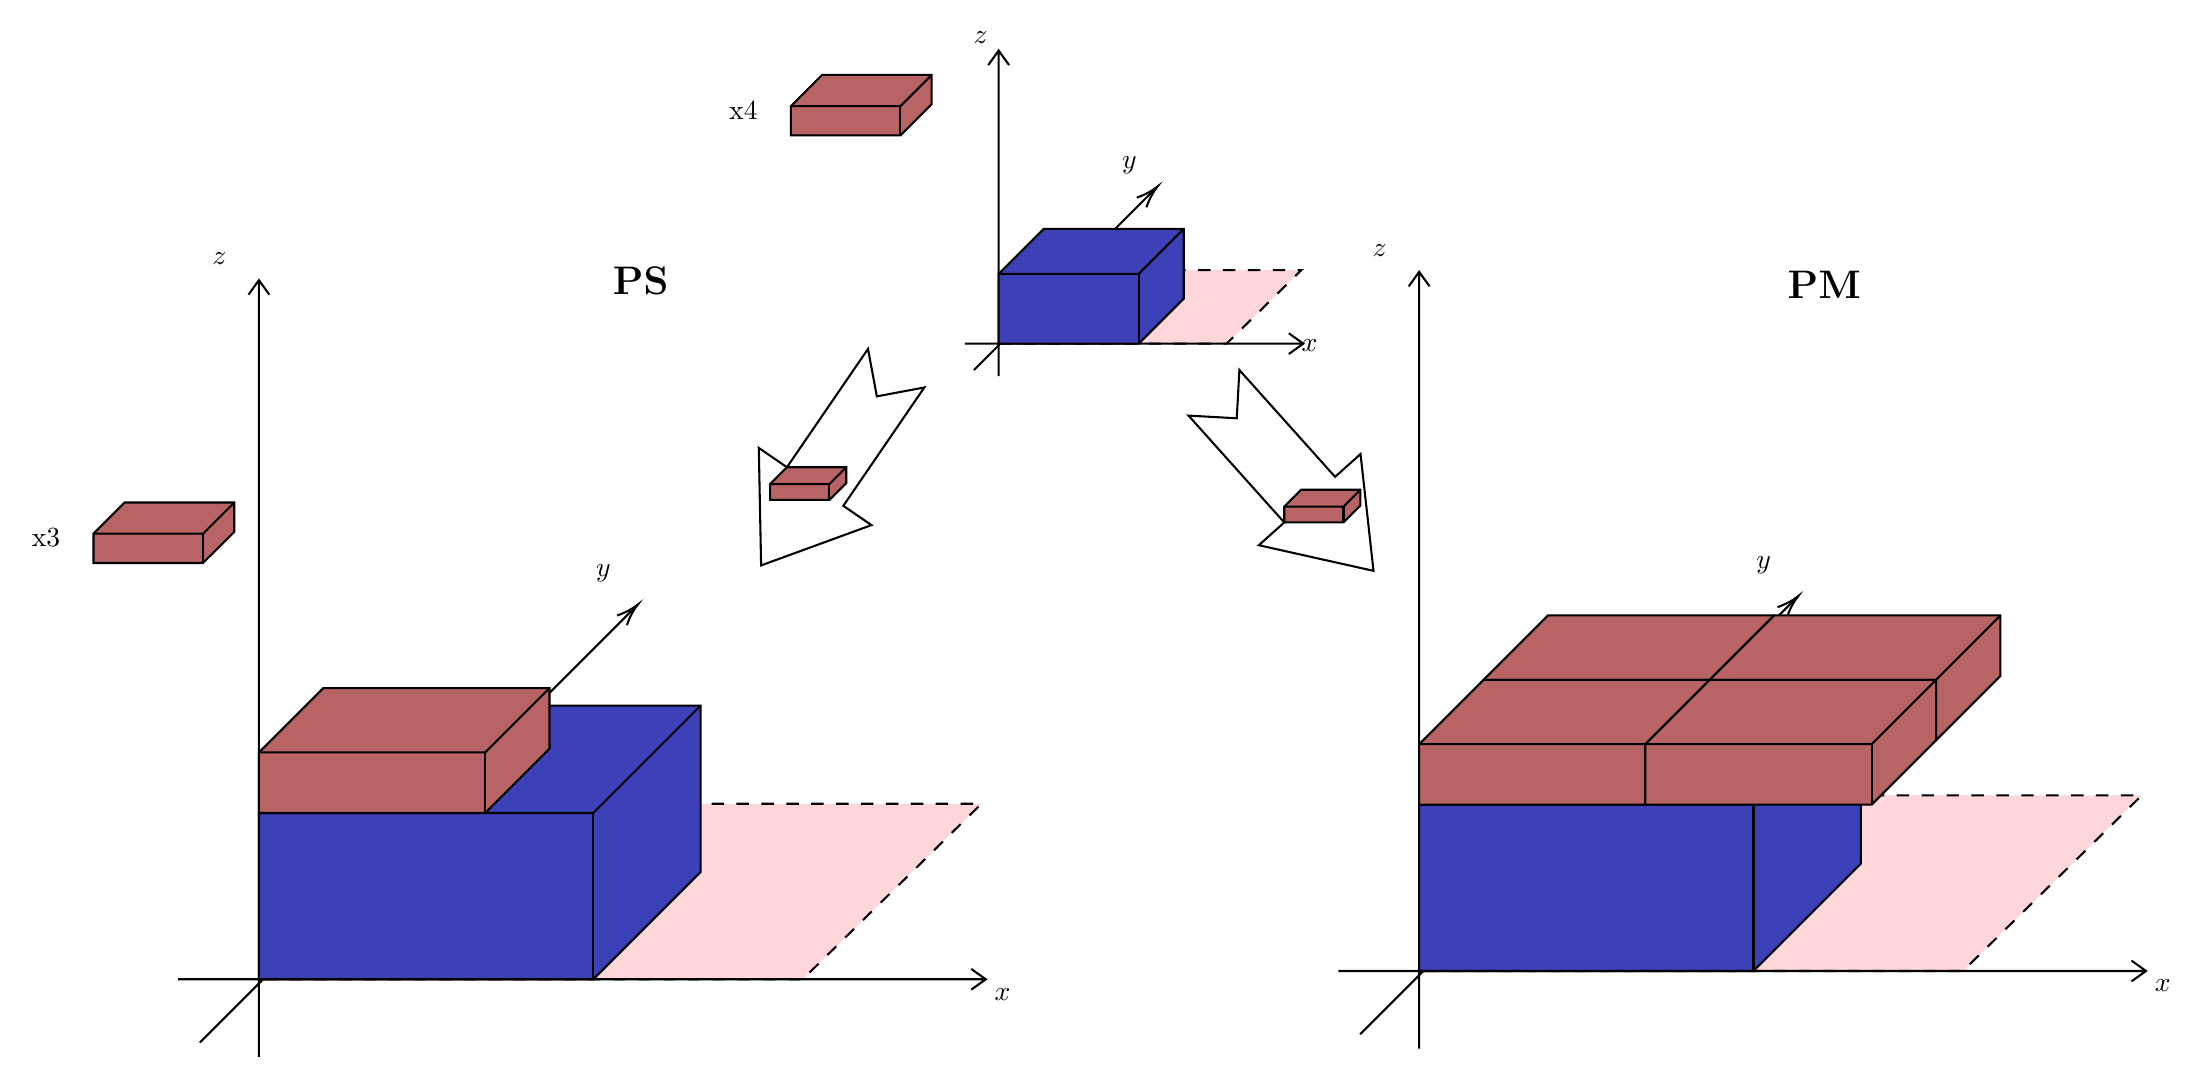
\begin{tikzpicture}[x=0.75pt,y=0.75pt,yscale=-1,xscale=1]
%uncomment if require: \path (0,561); %set diagram left start at 0, and has height of 561

%Shape: Parallelogram [id:dp6130378597775448] 
\draw  [fill={rgb, 255:red, 255; green, 17; blue, 34 }  ,fill opacity=0.17 ][dash pattern={on 4.5pt off 4.5pt}] (229,388) -- (491,388) -- (404.91,472.57) -- (142.91,472.57) -- cycle ;
%Shape: Axis 2D [id:dp62613490285975] 
\draw  (104,472.57) -- (493.11,472.57)(142.91,135.72) -- (142.91,510) (486.11,467.57) -- (493.11,472.57) -- (486.11,477.57) (137.91,142.72) -- (142.91,135.72) -- (147.91,142.72)  ;
%Straight Lines [id:da24042249863801912] 
\draw    (114.47,503.02) -- (324.19,293.3) ;
\draw [shift={(325.6,291.89)}, rotate = 135] [color={rgb, 255:red, 0; green, 0; blue, 0 }  ][line width=0.75]    (10.93,-3.29) .. controls (6.95,-1.4) and (3.31,-0.3) .. (0,0) .. controls (3.31,0.3) and (6.95,1.4) .. (10.93,3.29)   ;
%Shape: Cube [id:dp827644940904213] 
\draw  [fill={rgb, 255:red, 61; green, 65; blue, 184 }  ,fill opacity=1 ] (142.91,392.44) -- (194.61,340.75) -- (355.7,340.75) -- (355.7,420.88) -- (304,472.57) -- (142.91,472.57) -- cycle ; \draw   (355.7,340.75) -- (304,392.44) -- (142.91,392.44) ; \draw   (304,392.44) -- (304,472.57) ;
%Shape: Cube [id:dp9766511497579198] 
\draw  [fill={rgb, 255:red, 184; green, 100; blue, 100 }  ,fill opacity=1 ] (142.91,363.28) -- (173.91,332.28) -- (282.93,332.28) -- (282.93,361.44) -- (251.93,392.44) -- (142.91,392.44) -- cycle ; \draw   (282.93,332.28) -- (251.93,363.28) -- (142.91,363.28) ; \draw   (251.93,363.28) -- (251.93,392.44) ;
%Shape: Parallelogram [id:dp8629095007475812] 
\draw  [fill={rgb, 255:red, 255; green, 17; blue, 34 }  ,fill opacity=0.17 ][dash pattern={on 4.5pt off 4.5pt}] (535.39,130.86) -- (645.21,130.86) -- (609.13,166.31) -- (499.31,166.31) -- cycle ;
%Shape: Axis 2D [id:dp8379683853259726] 
\draw  (483,166.31) -- (646.1,166.31)(499.31,25.12) -- (499.31,182) (639.1,161.31) -- (646.1,166.31) -- (639.1,171.31) (494.31,32.12) -- (499.31,25.12) -- (504.31,32.12)  ;
%Straight Lines [id:da5442459432402652] 
\draw    (487.39,179.07) -- (574.47,91.99) ;
\draw [shift={(575.89,90.58)}, rotate = 135] [color={rgb, 255:red, 0; green, 0; blue, 0 }  ][line width=0.75]    (10.93,-3.29) .. controls (6.95,-1.4) and (3.31,-0.3) .. (0,0) .. controls (3.31,0.3) and (6.95,1.4) .. (10.93,3.29)   ;
%Shape: Cube [id:dp37678418294420923] 
\draw  [fill={rgb, 255:red, 61; green, 65; blue, 184 }  ,fill opacity=1 ] (499.31,132.72) -- (520.98,111.06) -- (588.5,111.06) -- (588.5,144.64) -- (566.83,166.31) -- (499.31,166.31) -- cycle ; \draw   (588.5,111.06) -- (566.83,132.72) -- (499.31,132.72) ; \draw   (566.83,132.72) -- (566.83,166.31) ;
%Notched Right Arrow [id:dp3073012233082779] 
\draw   (463.51,187.44) -- (424.47,244.46) -- (438.04,253.75) -- (384.87,273.17) -- (383.75,216.57) -- (397.32,225.87) -- (436.36,168.86) -- (440.64,191.72) -- cycle ;
%Shape: Cube [id:dp7783028256027571] 
\draw  [fill={rgb, 255:red, 184; green, 100; blue, 100 }  ,fill opacity=1 ] (389.2,233.99) -- (397.32,225.87) -- (425.88,225.87) -- (425.88,233.51) -- (417.76,241.63) -- (389.2,241.63) -- cycle ; \draw   (425.88,225.87) -- (417.76,233.99) -- (389.2,233.99) ; \draw   (417.76,233.99) -- (417.76,241.63) ;
%Shape: Parallelogram [id:dp6171754447847807] 
\draw  [fill={rgb, 255:red, 255; green, 17; blue, 34 }  ,fill opacity=0.17 ][dash pattern={on 4.5pt off 4.5pt}] (788,384) -- (1050,384) -- (963.91,468.57) -- (701.91,468.57) -- cycle ;
%Shape: Axis 2D [id:dp7940212818164142] 
\draw  (663,468.57) -- (1052.11,468.57)(701.91,131.72) -- (701.91,506) (1045.11,463.57) -- (1052.11,468.57) -- (1045.11,473.57) (696.91,138.72) -- (701.91,131.72) -- (706.91,138.72)  ;
%Straight Lines [id:da8066729156616194] 
\draw    (673.47,499.02) -- (883.19,289.3) ;
\draw [shift={(884.6,287.89)}, rotate = 135] [color={rgb, 255:red, 0; green, 0; blue, 0 }  ][line width=0.75]    (10.93,-3.29) .. controls (6.95,-1.4) and (3.31,-0.3) .. (0,0) .. controls (3.31,0.3) and (6.95,1.4) .. (10.93,3.29)   ;
%Shape: Cube [id:dp35418890536629477] 
\draw  [fill={rgb, 255:red, 61; green, 65; blue, 184 }  ,fill opacity=1 ] (701.91,388.44) -- (753.61,336.75) -- (914.7,336.75) -- (914.7,416.88) -- (863,468.57) -- (701.91,468.57) -- cycle ; \draw   (914.7,336.75) -- (863,388.44) -- (701.91,388.44) ; \draw   (863,388.44) -- (863,468.57) ;
%Notched Right Arrow [id:dp17687615727785144] 
\draw   (615.3,179.04) -- (661.41,230.5) -- (673.66,219.51) -- (679.91,275.78) -- (624.66,263.44) -- (636.91,252.46) -- (590.8,201) -- (614.03,202.27) -- cycle ;
%Shape: Cube [id:dp6377400416878792] 
\draw  [fill={rgb, 255:red, 184; green, 100; blue, 100 }  ,fill opacity=1 ] (636.91,244.82) -- (645.03,236.7) -- (673.59,236.7) -- (673.59,244.34) -- (665.47,252.46) -- (636.91,252.46) -- cycle ; \draw   (673.59,236.7) -- (665.47,244.82) -- (636.91,244.82) ; \draw   (665.47,244.82) -- (665.47,252.46) ;
%Shape: Cube [id:dp144413986349461] 
\draw  [fill={rgb, 255:red, 184; green, 100; blue, 100 }  ,fill opacity=1 ] (399.2,51.88) -- (414.21,36.87) -- (467.01,36.87) -- (467.01,50.99) -- (451.99,66) -- (399.2,66) -- cycle ; \draw   (467.01,36.87) -- (451.99,51.88) -- (399.2,51.88) ; \draw   (451.99,51.88) -- (451.99,66) ;
%Shape: Cube [id:dp7037511540247638] 
\draw  [fill={rgb, 255:red, 184; green, 100; blue, 100 }  ,fill opacity=1 ] (63.2,257.88) -- (78.21,242.87) -- (131.01,242.87) -- (131.01,256.99) -- (115.99,272) -- (63.2,272) -- cycle ; \draw   (131.01,242.87) -- (115.99,257.88) -- (63.2,257.88) ; \draw   (115.99,257.88) -- (115.99,272) ;
%Shape: Cube [id:dp9586193782273413] 
\draw  [fill={rgb, 255:red, 184; green, 100; blue, 100 }  ,fill opacity=1 ] (732.91,328.28) -- (763.91,297.28) -- (872.93,297.28) -- (872.93,326.44) -- (841.93,357.44) -- (732.91,357.44) -- cycle ; \draw   (872.93,297.28) -- (841.93,328.28) -- (732.91,328.28) ; \draw   (841.93,328.28) -- (841.93,357.44) ;
%Shape: Cube [id:dp710841498210852] 
\draw  [fill={rgb, 255:red, 184; green, 100; blue, 100 }  ,fill opacity=1 ] (841.93,328.28) -- (872.93,297.28) -- (981.95,297.28) -- (981.95,326.44) -- (950.95,357.44) -- (841.93,357.44) -- cycle ; \draw   (981.95,297.28) -- (950.95,328.28) -- (841.93,328.28) ; \draw   (950.95,328.28) -- (950.95,357.44) ;
%Shape: Cube [id:dp6597094389022091] 
\draw  [fill={rgb, 255:red, 184; green, 100; blue, 100 }  ,fill opacity=1 ] (701.91,359.28) -- (732.91,328.28) -- (841.93,328.28) -- (841.93,357.44) -- (810.93,388.44) -- (701.91,388.44) -- cycle ; \draw   (841.93,328.28) -- (810.93,359.28) -- (701.91,359.28) ; \draw   (810.93,359.28) -- (810.93,388.44) ;
%Shape: Cube [id:dp329793740757924] 
\draw  [fill={rgb, 255:red, 184; green, 100; blue, 100 }  ,fill opacity=1 ] (810.93,359.28) -- (841.93,328.28) -- (950.95,328.28) -- (950.95,357.44) -- (919.95,388.44) -- (810.93,388.44) -- cycle ; \draw   (950.95,328.28) -- (919.95,359.28) -- (810.93,359.28) ; \draw   (919.95,359.28) -- (919.95,388.44) ;

% Text Node
\draw (303.9,271.2) node [anchor=north west][inner sep=0.75pt]    {$y$};
% Text Node
\draw (495.84,475.35) node [anchor=north west][inner sep=0.75pt]    {$x$};
% Text Node
\draw (118.94,121.14) node [anchor=north west][inner sep=0.75pt]    {$z$};
% Text Node
\draw (312,128) node [anchor=north west][inner sep=0.75pt]  [font=\Large] [align=left] {\textbf{PS}};
% Text Node
\draw (557.3,74.49) node [anchor=north west][inner sep=0.75pt]    {$y$};
% Text Node
\draw (643.76,163.06) node [anchor=north west][inner sep=0.75pt]    {$x$};
% Text Node
\draw (485.78,14.59) node [anchor=north west][inner sep=0.75pt]    {$z$};
% Text Node
\draw (862.9,267.2) node [anchor=north west][inner sep=0.75pt]    {$y$};
% Text Node
\draw (1054.84,471.35) node [anchor=north west][inner sep=0.75pt]    {$x$};
% Text Node
\draw (677.94,117.14) node [anchor=north west][inner sep=0.75pt]    {$z$};
% Text Node
\draw (878,130) node [anchor=north west][inner sep=0.75pt]  [font=\Large] [align=left] {\textbf{PM}};
% Text Node
\draw (368,48) node [anchor=north west][inner sep=0.75pt]   [align=left] {x4};
% Text Node
\draw (32,254) node [anchor=north west][inner sep=0.75pt]   [align=left] {x3};


\end{tikzpicture}
